%!TEX root = ../../../main.tex
%%---------------------------------------------------------------------------
\section{Vision}
\label{sec:rc_hmi_sec}
%%---------------------------------------------------------------------------
Position and rotation description of the bricks \\


	\begin{figure}[H]
		\centering
	    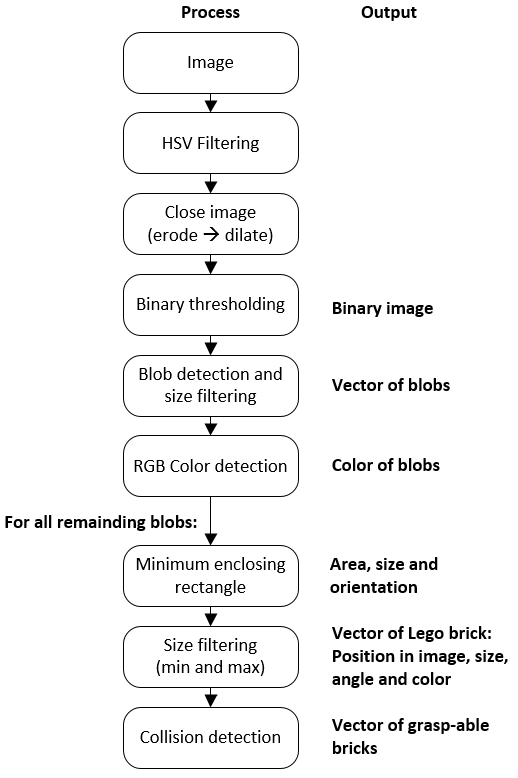
\includegraphics[width=0.7\textwidth]{rc_vision_steps}
	    \caption{Steps to be performed when an image is searched for Lego bricks}
		\label{fig:rc_vision_steps}
	\end{figure}
	
	\begin{figure}[H]
		\centering
	    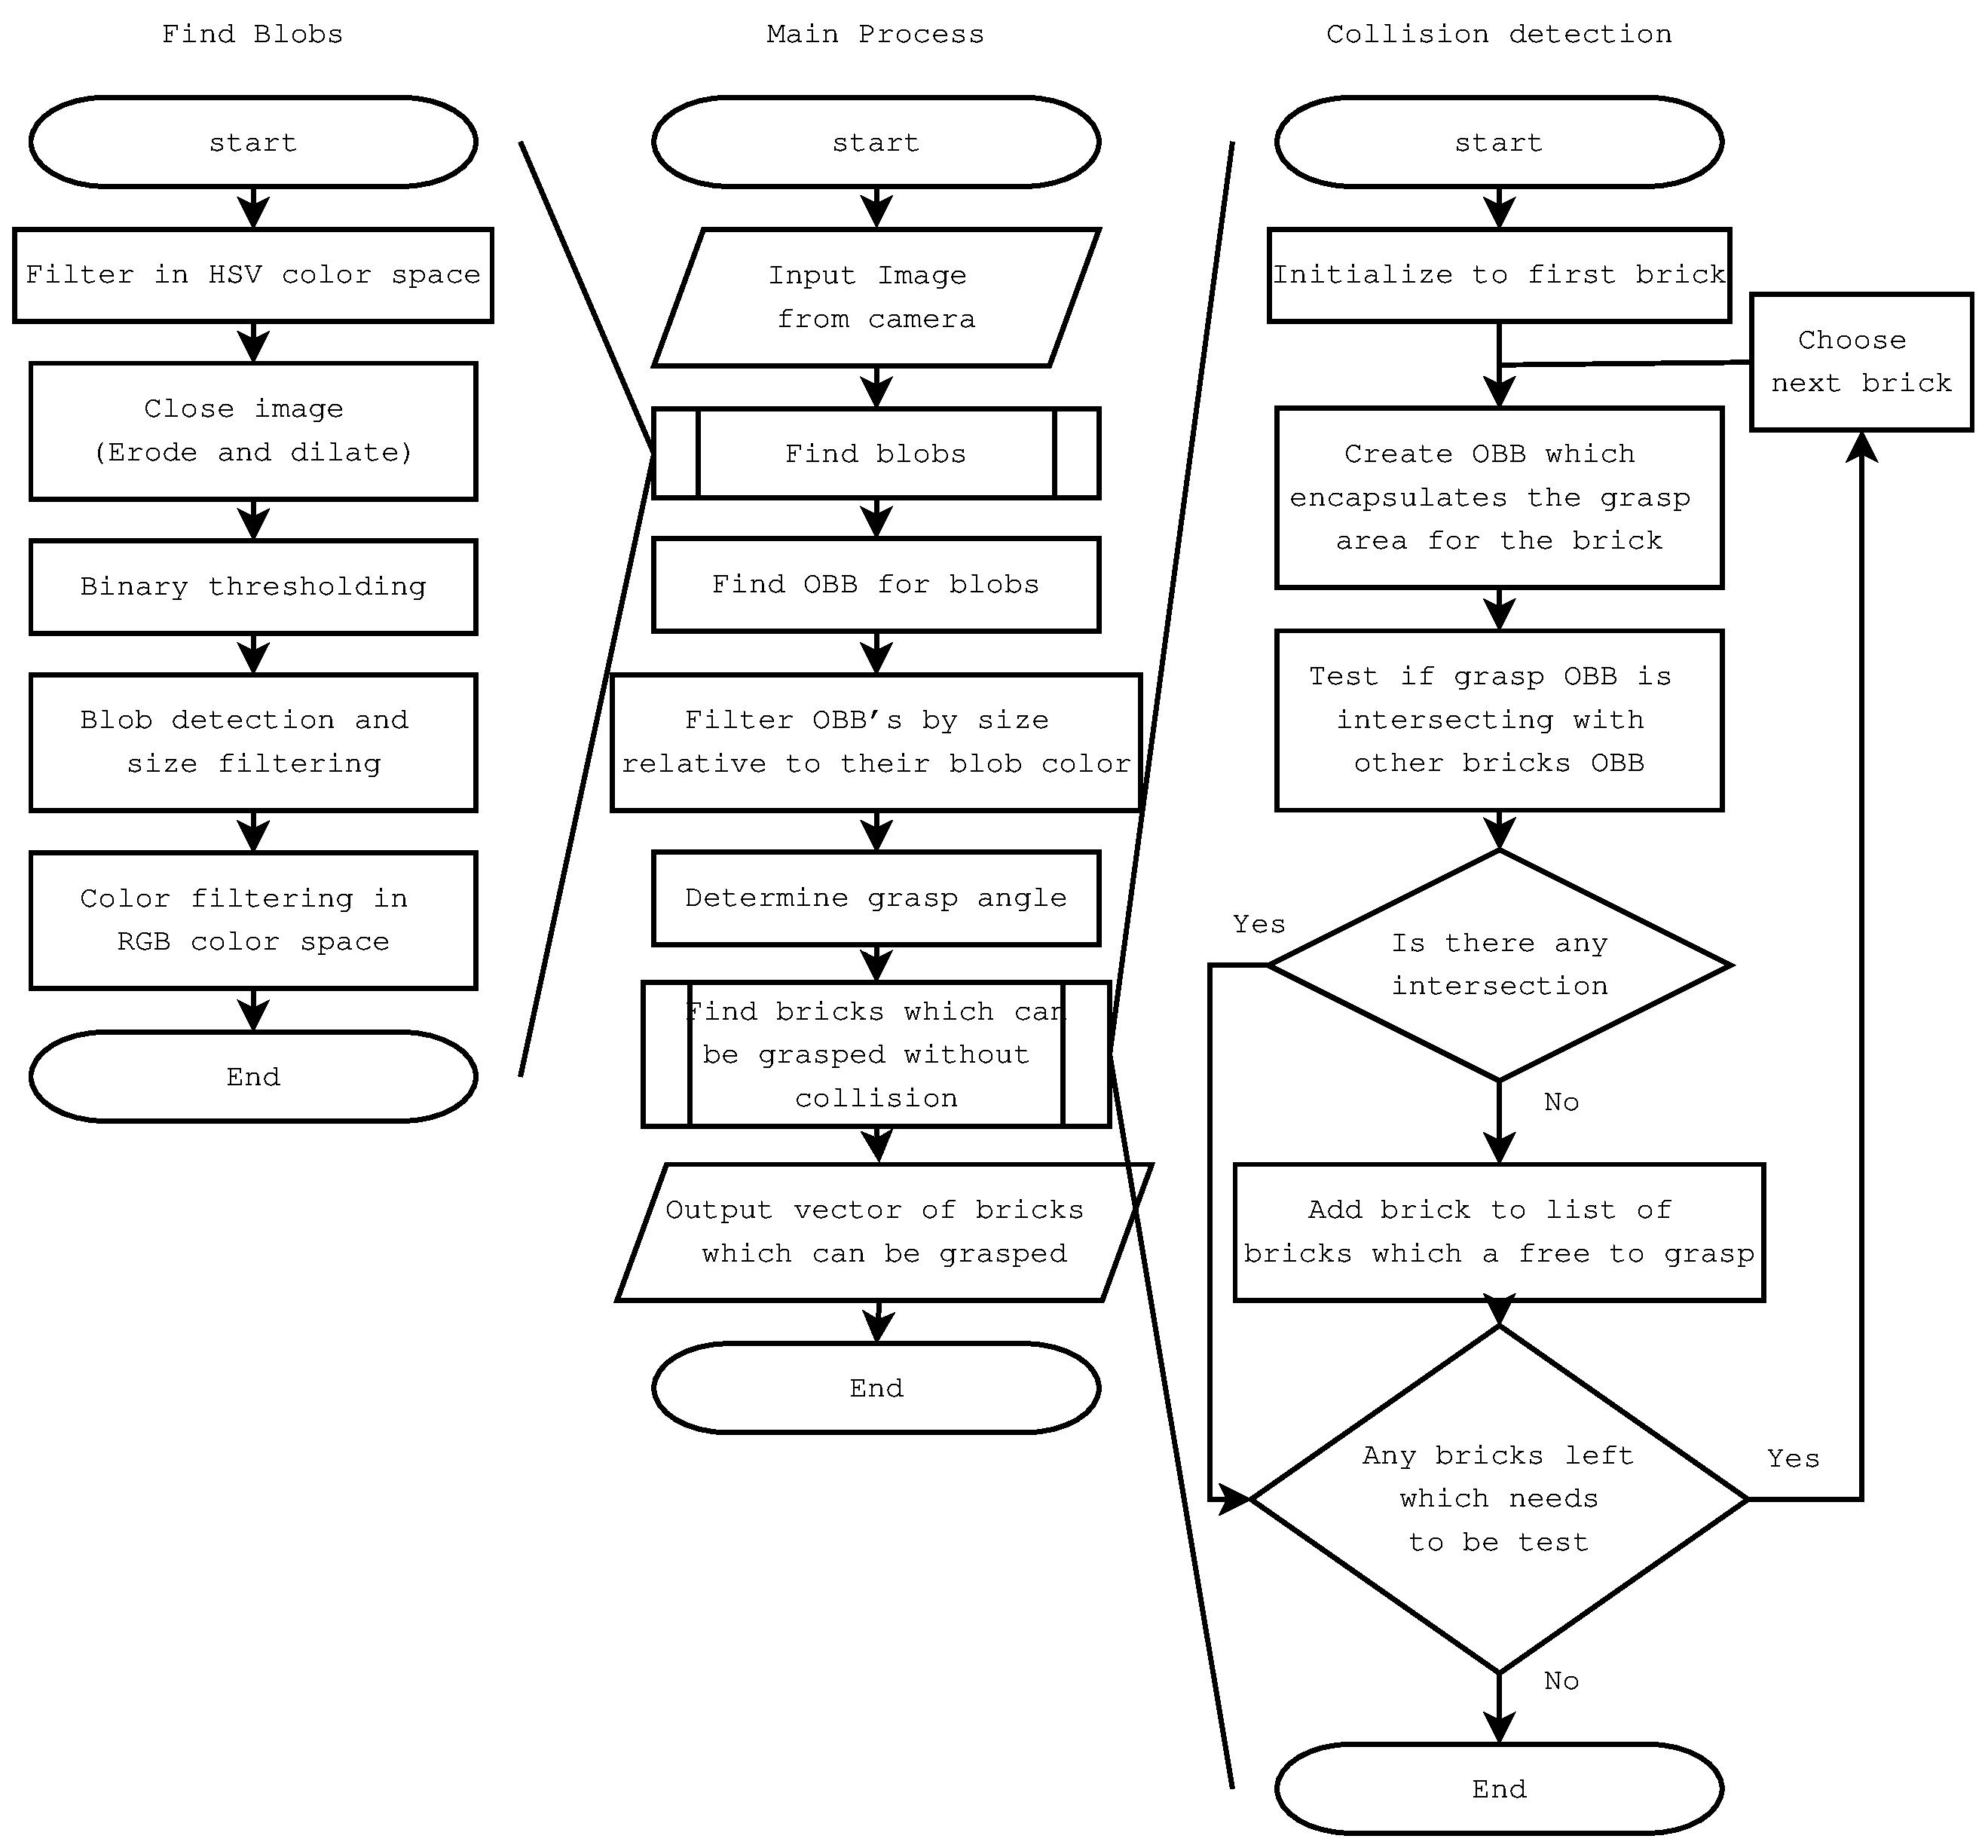
\includegraphics[width=0.8\textwidth]{rc_vision_thor.eps}
	    \caption{Steps to be performed when an image is searched for Lego bricks}
		\label{fig:rc_vision_steps_thor}
	\end{figure}
	
	\begin{figure}[H]
		\centering
	    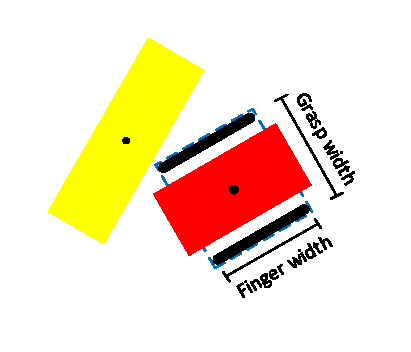
\includegraphics[width=0.6\textwidth]{rc_vision_collision}
	    \caption{Lego brick collision detection method}
		\label{fig:rc_vision_collision}
	\end{figure}
	
Collision avoidance is done by testing if any obstacles is in the grasp path for a brick. The grasp path for a brick is the area the two fingers of the end effector travels when trying to grasp the brick. Figure \ref{fig:rc_vision_collision} shows a example where the two bold black lines illustrates the end effector fingers. The area encapsulated by the stripped blue lines is the grasp path area for the grasp when trying to grasp the red brick illustrated by a red rectangle. A grasp path area is then tested against all other bricks except the brick to be grasped. Separating axis theorem\cite{Gottschalk:1996:OHS:237170.237244} is used to test if the rectangular grasp area is colliding with the rectangular brick areas defined by OBB's.